\documentclass[leqno,twocolumn]{article}
\usepackage[margin=0.5in]{geometry}
\usepackage[utf8]{inputenc}
\usepackage{amsmath, amsfonts, color, booktabs, centernot, graphicx, fancyhdr}
\usepackage[linktoc=all,hidelinks]{hyperref}
\setlength\parindent{0pt}
\begin{document}
\onecolumn
\title{Journal of Fall 2014}
\author{Leah Dickstein}

\maketitle

\tableofcontents

\section{Nonlinear Memoryless Control: Tangent Line Approximation--Incorrect?}

\begin{align*}
x(n) &= ax(n-1) + w(n-1)\\
y(n) &= cx^2(n) + v1(n)\\
y'(n) &= \alpha(n) x(n) + \beta(n) \\
\hat{x}(n) &= fy'(n) + g\\
{} \\
min \mathbb{E}[||X - \hat{X}||^2] &= \mathbb{E}[||x(n) - fy'(n) - g||^2]\\
{} \\
\frac{d}{df} \: \mathbb{E}[||x(n) - fy'(n) - g||^2] &= \mathbb{E}[2(x(n) - fy'(n) - g)(-y'(n))] = 0\\
&= \mathbb{E}[-x(n)y'(n) + fy'^2(n) + gy'(n)] = 0\\
f\mathbb{E}[y'^2(n)] &= \mathbb{E}[x(n)y'(n)] - g\mathbb{E}[y'(n)]\\
{} \\
\frac{d}{dg} \: \mathbb{E}[||x(n) - fy'(n) - g||^2] &= \mathbb{E}[2(x(n) - fy'(n) - g)(-1)] = 0\\
& \mathbb{E}[-x(n) + fy'(n) + g] = 0\\
g &= \mathbb{E}[x(n) - fy'(n)]\\
{} \\
f \mathbb{E}[y'^2(n)] &= \mathbb{E}[x(n)y'(n)] - \mathbb{E}[y'(n)] \mathbb{E}[x(n) - fy'(n)] \\
f (\mathbb{E}[y'^2(n)] - (\mathbb{E}[y'(n)])^2 ) &= \mathbb{E}[x(n)y'(n)] - \mathbb{E}[x(n)] \mathbb{E}[y'(n)] \\
f &= \frac{cov(x(n), y(n) )}{var(y'(n))}\\
{} \\
\hat{X}(n) &= \frac{cov(x(n), y(n) )}{var(y'(n))} (y'(n) - \mathbb{E}[y'(n)] + \mathbb{E}[x(n)]
\end{align*}


Assuming $\alpha(n)$ and $\beta(n)$ are constants for a given $n$:
\begin{align*}
\mathbb{E}[x(n) (\alpha x(n) + \beta)] - \mathbb{E}[x(n)] \mathbb{E}[\alpha x(n) + \beta ] &= \alpha \mathbb{E}[x^2(n)] + \beta \mathbb{E}[x(n)] - \alpha (\mathbb{E}[x(n)])^2 - \beta \mathbb{E}[x(n)] \\
&= \alpha \mathbb{E}[x^2(n)] - \alpha (\mathbb{E}[x(n)])^2 \\
&= \alpha Var(x(n))\\
{}\\
\mathbb{E}[(\alpha x(n) + \beta)^2 ] - (\mathbb{E}[\alpha x(n) + \beta ])^2 &= \mathbb{E}[\alpha^2 x^2(n) + 2\alpha \beta x(n) + \beta^2] - \mathbb{E}[\alpha x(n) + \beta] \mathbb{E}[\alpha x(n) + \beta] \\
&= \alpha^2 \mathbb{E}[x^2(n)] + 2 \alpha \beta \mathbb{E}[x(n)] + \beta^2 - \alpha^2 (\mathbb{E}[x(n)])^2 - 2 \alpha \beta \mathbb{E}[x(n)] - \beta^2 \\
&= \alpha^2 \mathbb{E}[x^2(n)] - \alpha^2 (\mathbb{E}[x(n)])^2 \\
&= \alpha^2 Var(x(n))\\
{} \\
L[X(n) | Y(n)] &= \frac{1}{\alpha} (Y(n) - \mathbb{E}[Y(n)]) + \mathbb{E}[X(n)]\\
&= \frac{Y(n) - \mathbb{E}[\alpha X(n) + \beta]}{\alpha} + \mathbb{E}[X(n)]\\
&= \frac{Y(n) - \beta}{\alpha}
\end{align*}

The calculation for $\alpha(n)$ and $\beta(n)$, if $y'$ is the function and $y'(n)$ is the realization of the function at timestep $n$:
\begin{align*}
\frac{dy}{dx} &= 2cx(n)\\
y' - y'(n) &= \frac{dy}{dx} (x - x(n))\\
y' &= \frac{dy}{dx} x + \left( y'(n) - \frac{dy}{dx} x(n) \right)\\
&= \alpha x + \beta\\
{} \\
\alpha &= 2cx(n)\\
\beta &= y'(n) - \alpha x(n)
\end{align*}

If I attempt to calculate the linear estimator after plugging in what $\alpha$ and $\beta$ are, I'll just get the linear estimator of X and Y (where Y is nonlinear, the estimator gave unbounded error.)

\section{"U" Delay}

System:
\begin{align*}
X(n+1) &= AX(n) + W(n) - U(n-k)\\
Y(n) &= C(n)\\
U(n) &= L[X(n)|Y(n)]\\
k &= 2
\end{align*}

Note in this system there is no observation noise! Delay = 2.

\begin{tabular*}{\textwidth}{c @{\extracolsep{\fill}} ccc}
$x(0) \sim N(\mu_{x[0]}, \sigma^2_{x[0]})$ & y(0) = cx(0) & u(0) = x(0)\\
$x(1) = ax(0) + w(0)$ & y(1) = cx(1) & u(1) = x(1)\\
$x(2) = a^2x(0) + aw(0) + w(1) - x(0)$ & y(2) = cx(2) & u(2) = x(2)
\end{tabular*}\\

Since we have perfect observation, the calculations for Y and U are obvious. I'm now going to focus on the evolution of X:\\

{\renewcommand{\arraystretch}{2}%
%{\setlength{\tabcolsep}{2em}
$\begin{array}{c|c|c|c|c|c|c|c|c|l|}
{} & x(0) & x(1) & x(2) & x(3) & x(4) & x(5) & x(6) & x(7) & \cdots\\
\hline
x(0) & 1 & a & a^2-1 & a^3 - 2a & a^4 - 3a^2 + 1 & a^5 - 4a^3 + 3a & a^6 - 5a^4 + 6a^2 -1 & a^7 - 6a^5 + 10a^3 - 4a & \cdots\\
w(0) & 0 & 1 & a & a^2-1 & a^3 - 2a & a^4 - 3a^2 + 1 & a^5 - 4a^3 + 3a & a^6 - 5a^4 + 6a^2 -1 & \cdots \\
w(1) & 0 & 0 & 1 & a & a^2-1 & a^3 - 2a & a^4 - 3a^2 + 1 & a^5 - 4a^3 + 3a & \cdots \\
w(2) & 0 & 0 & 0 & 1 & a & a^2-1 & a^3 - 2a & a^4 - 3a^2 + 1 & \cdots \\
w(3) & 0 & 0 & 0 & 0 & 1 & a & a^2-1 & a^3 - 2a & \cdots \\
w(4) & 0 & 0 & 0 & 0 & 0 & 1 & a & a^2-1 & \cdots \\
w(5) & 0 & 0 & 0 & 0 & 0 & 0 & 1 & a & \cdots \\
w(6) & 0 & 0 & 0 & 0 & 0 & 0 & 0 & 1 & \cdots \\
w(7) & 0 & 0 & 0 & 0 & 0 & 0 & 0 & 0 & \cdots\\
\vdots & 0 & 0 & 0 & 0 & 0 & 0 & 0 & 0 & \ddots
\end{array}$ \newline \newline

You can see that this forms a lower triangular matrix with exploding number of terms. Convolution??

The system is autoregressive with order $k$. For example, if delay $k = 2$, the system is represented by the following matrix:
\[ \left[ \begin{matrix}
x(1)\\ x(2) \\ \vdots
\end{matrix} \right] = \left[ \begin{matrix}
x(0) & x(-1)\\
x(1) & x(0)\\
\ddots & \ddots
\end{matrix} \right] \left[ \begin{matrix}
a \\ -1 \\ \vdots 
\end{matrix} \right] \]

\[X_t = c + \sum_{i=1}^{p} \phi_i X_{t-i} + \epsilon_t \]
\[X_t = \mu_{x[0]} + aX_{t-1} -1X_{t-2} + \epsilon_t \]

\subsection{Simulation}
We can see that if W = 0, smaller values of a still have bounded error. Here are some examples:

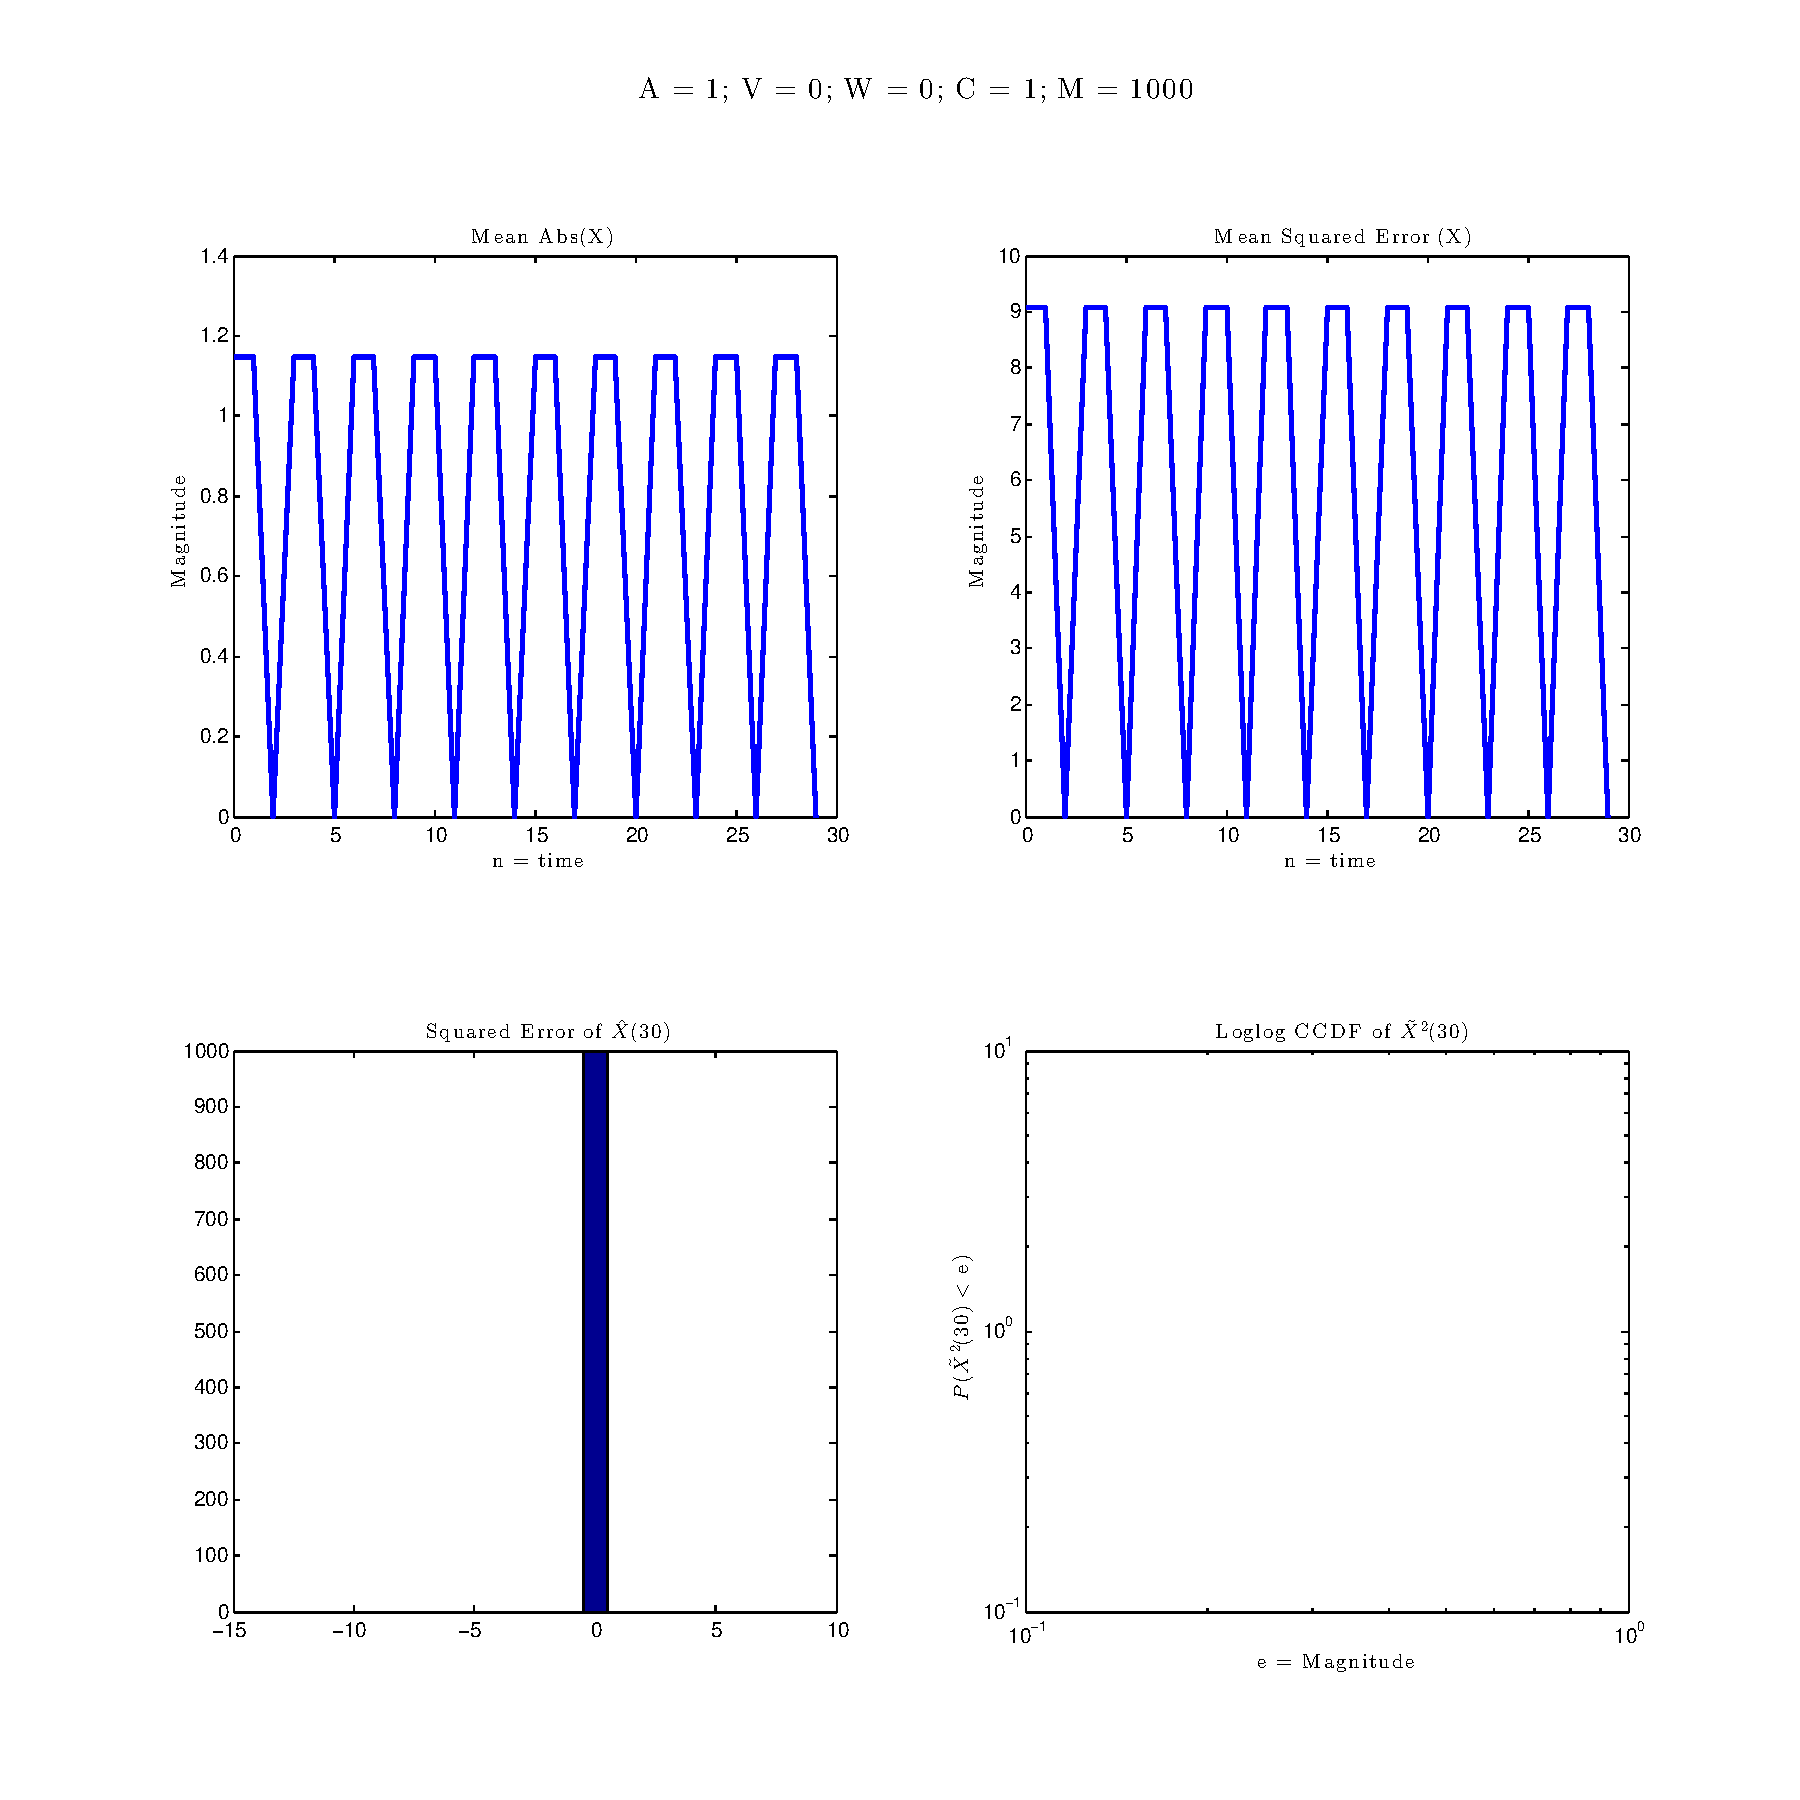
\includegraphics[width=0.5\textwidth]{udelay_0}
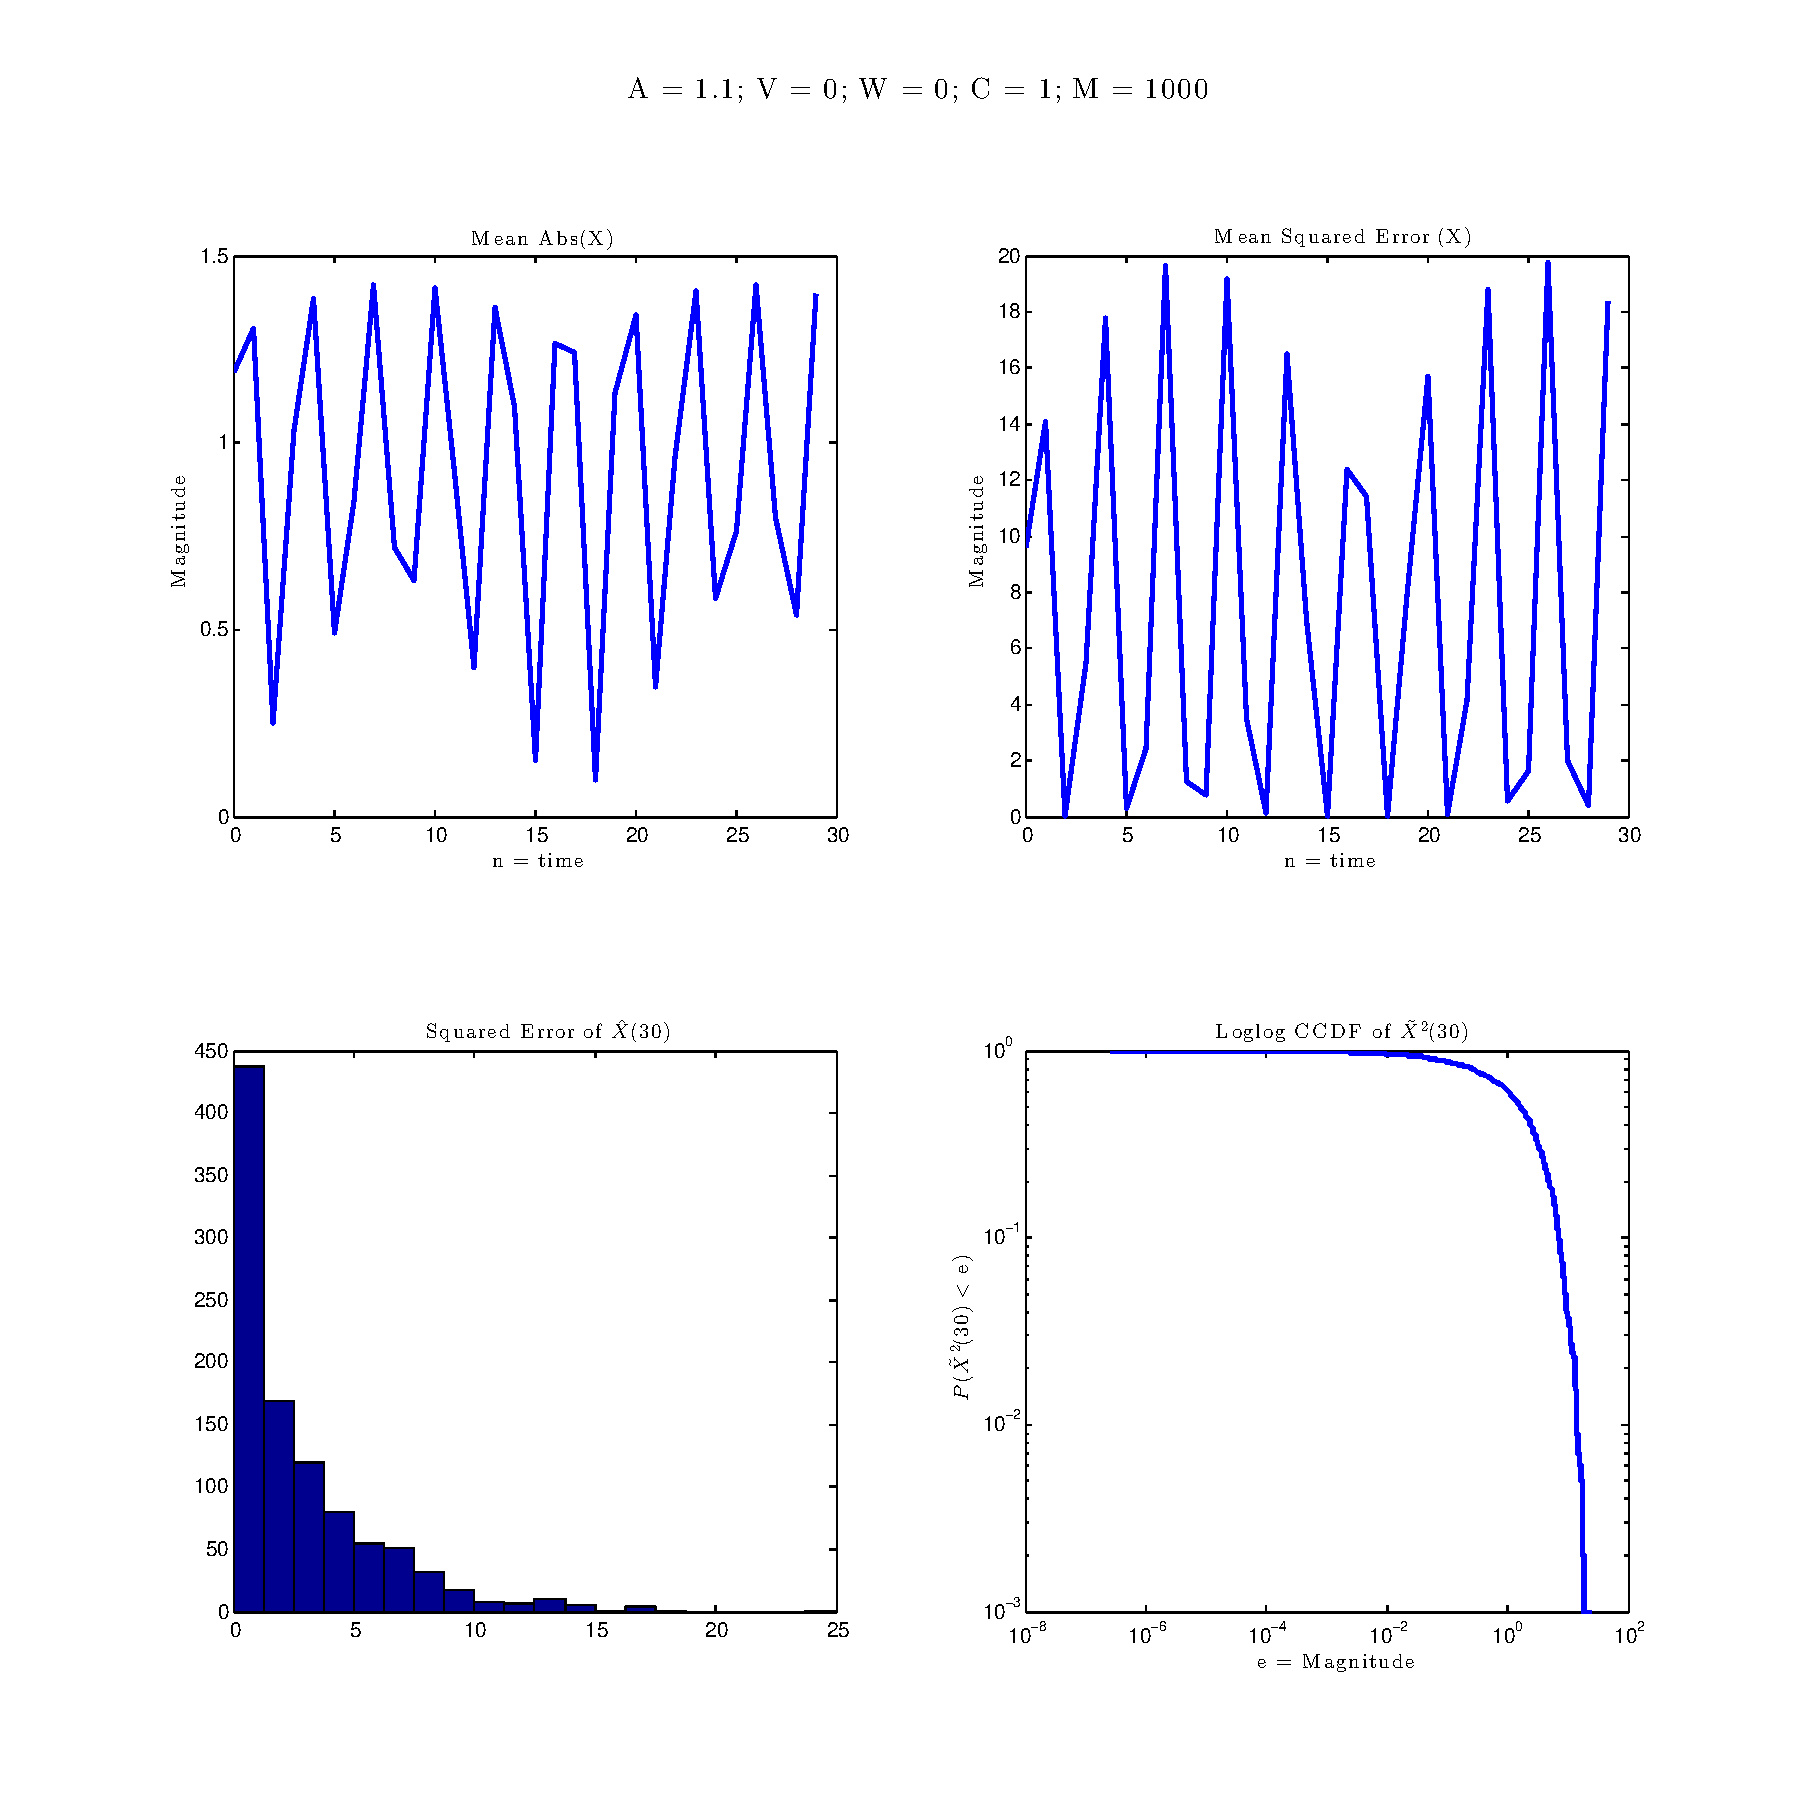
\includegraphics[width=0.5\textwidth]{udelay_1}\\
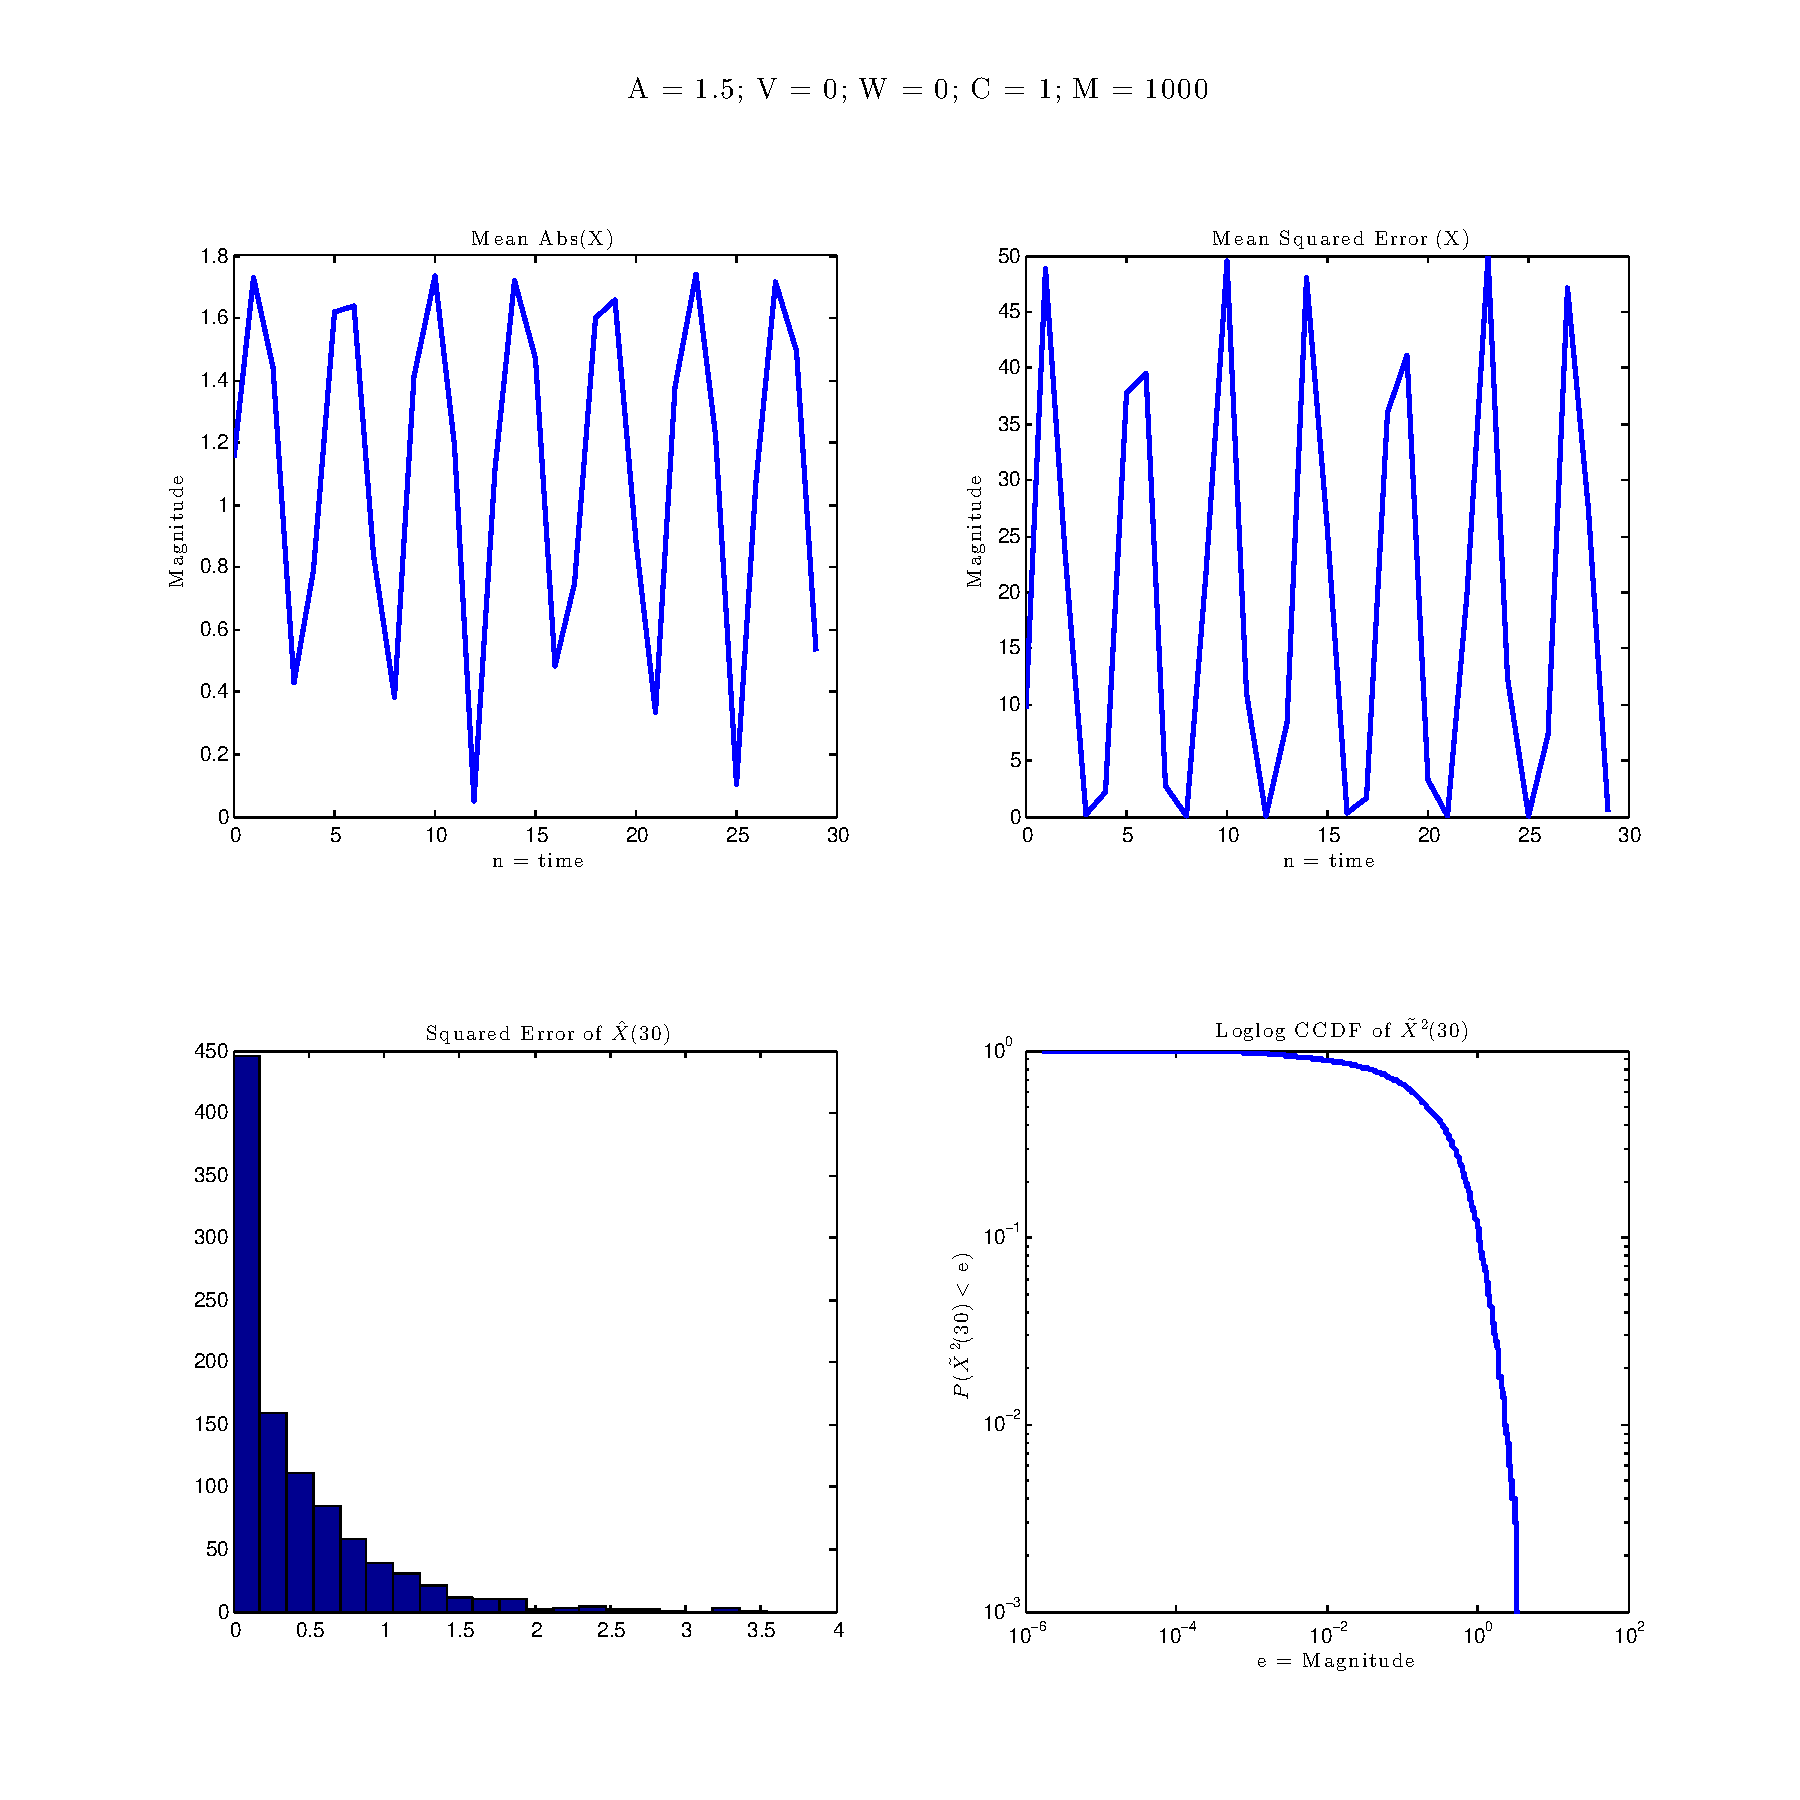
\includegraphics[width=0.5\textwidth]{udelay_2}


However when a is too large (here it's 2) the equations explode. 

\begin{center}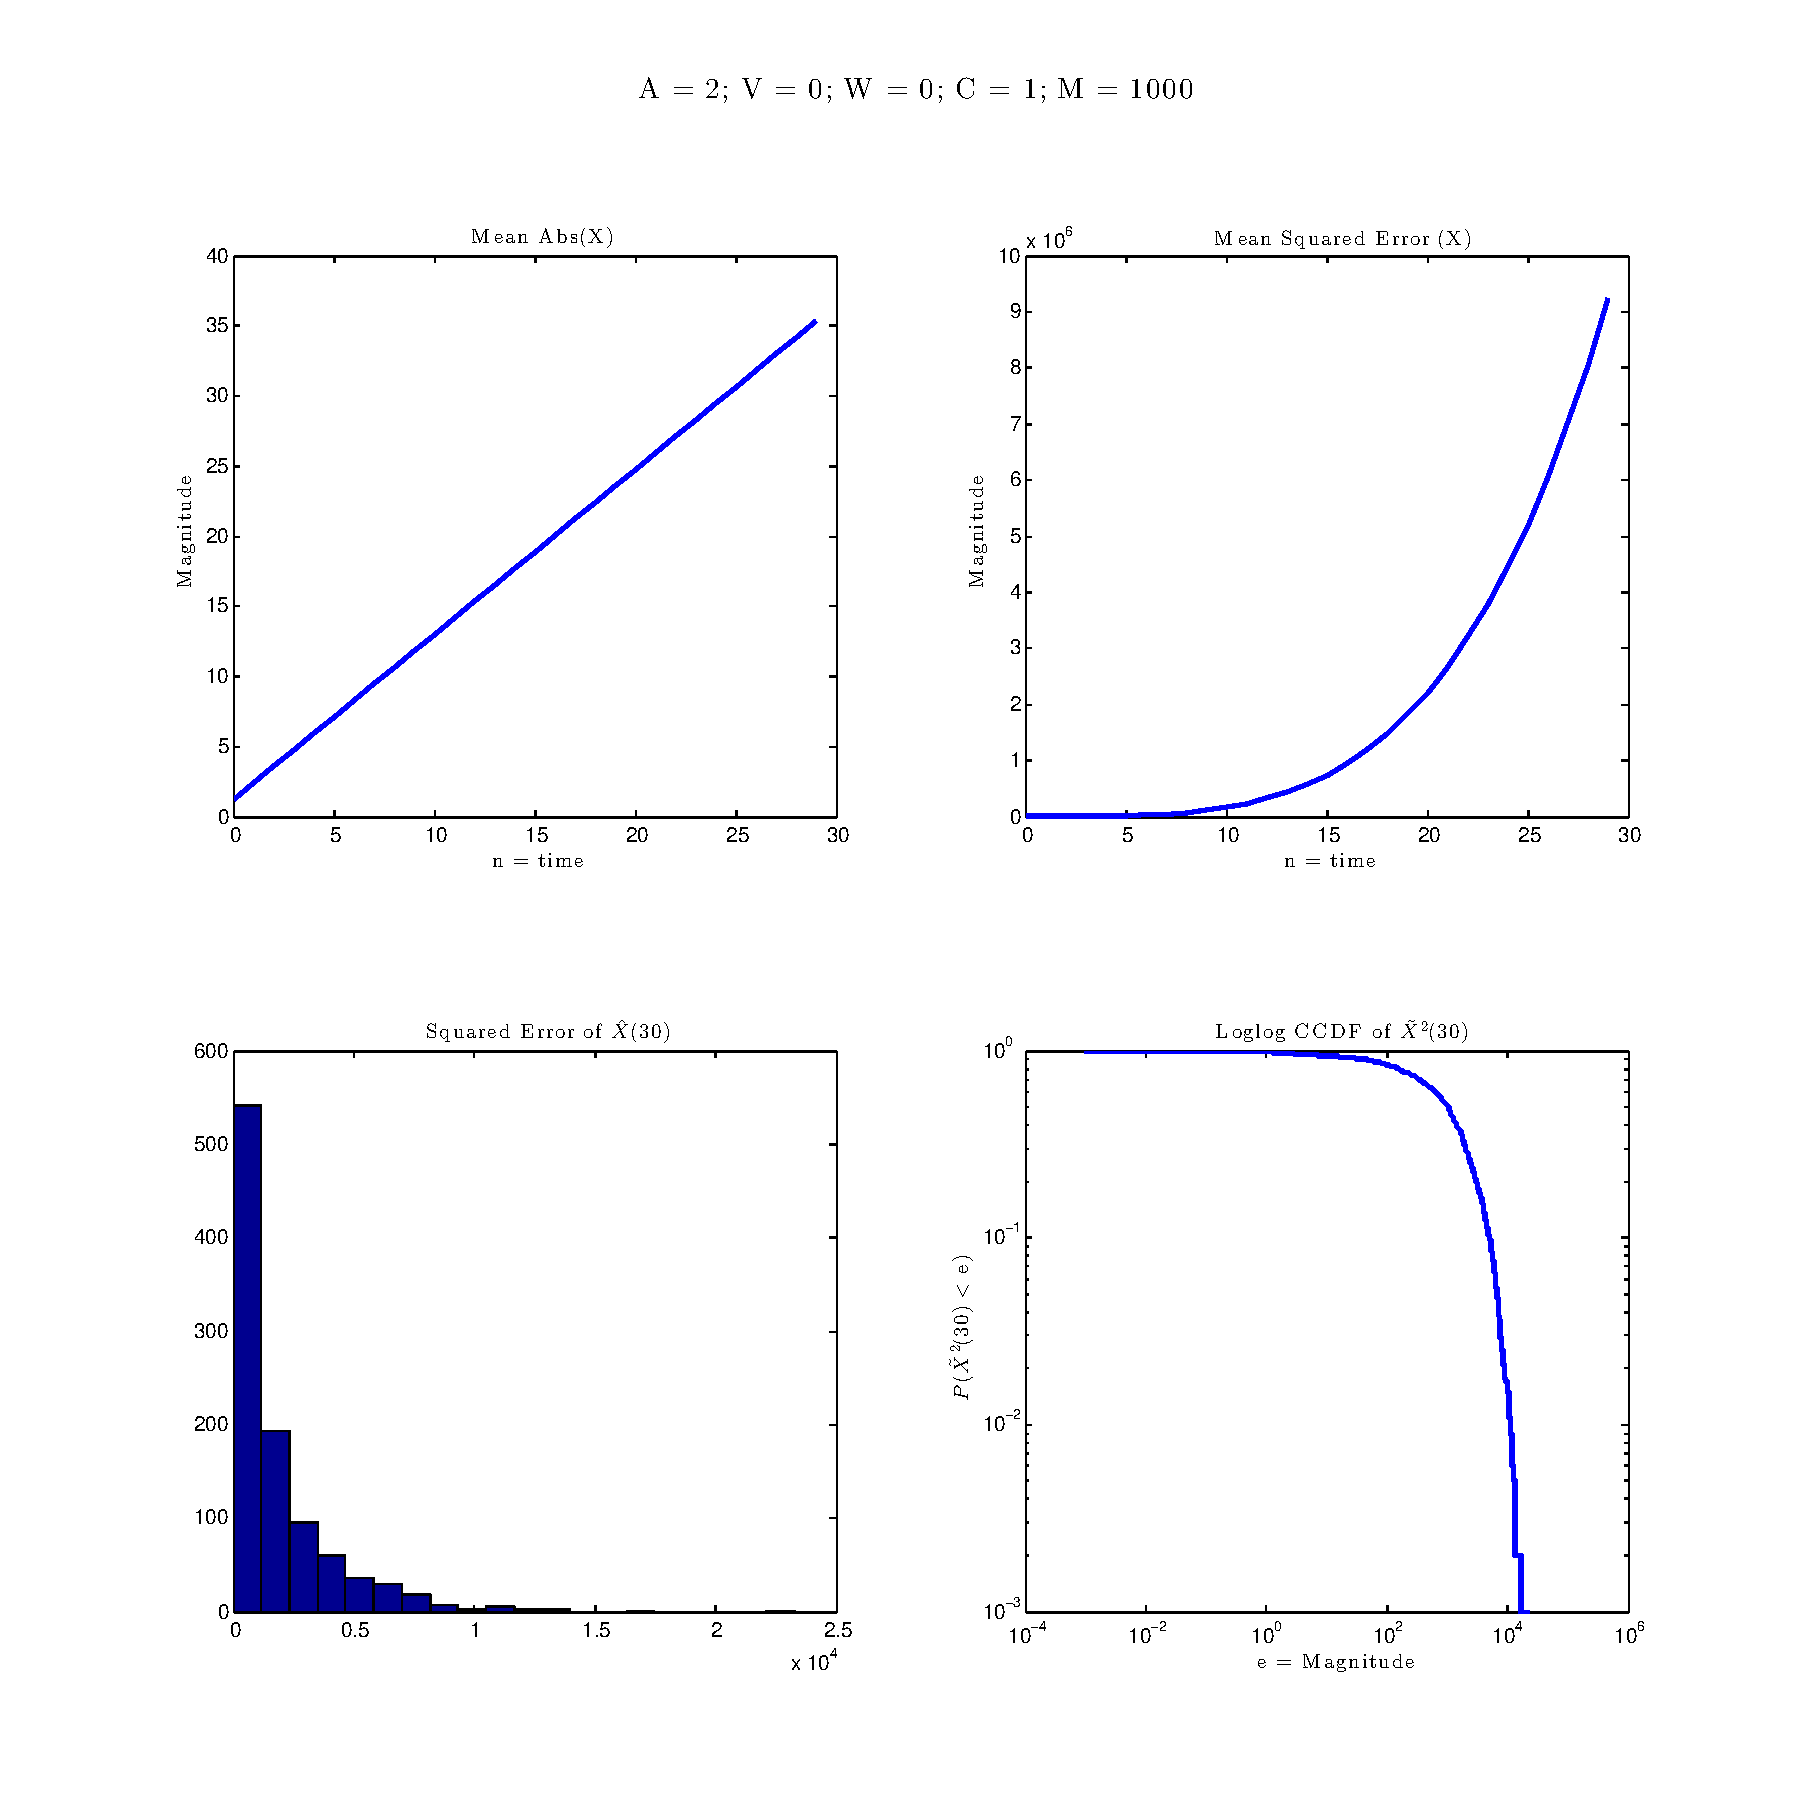
\includegraphics[width=0.5\textwidth]{udelay_3}\end{center}

Based on the numbers, a = 1 should produce something sinusoidal and it does:
\begin{center}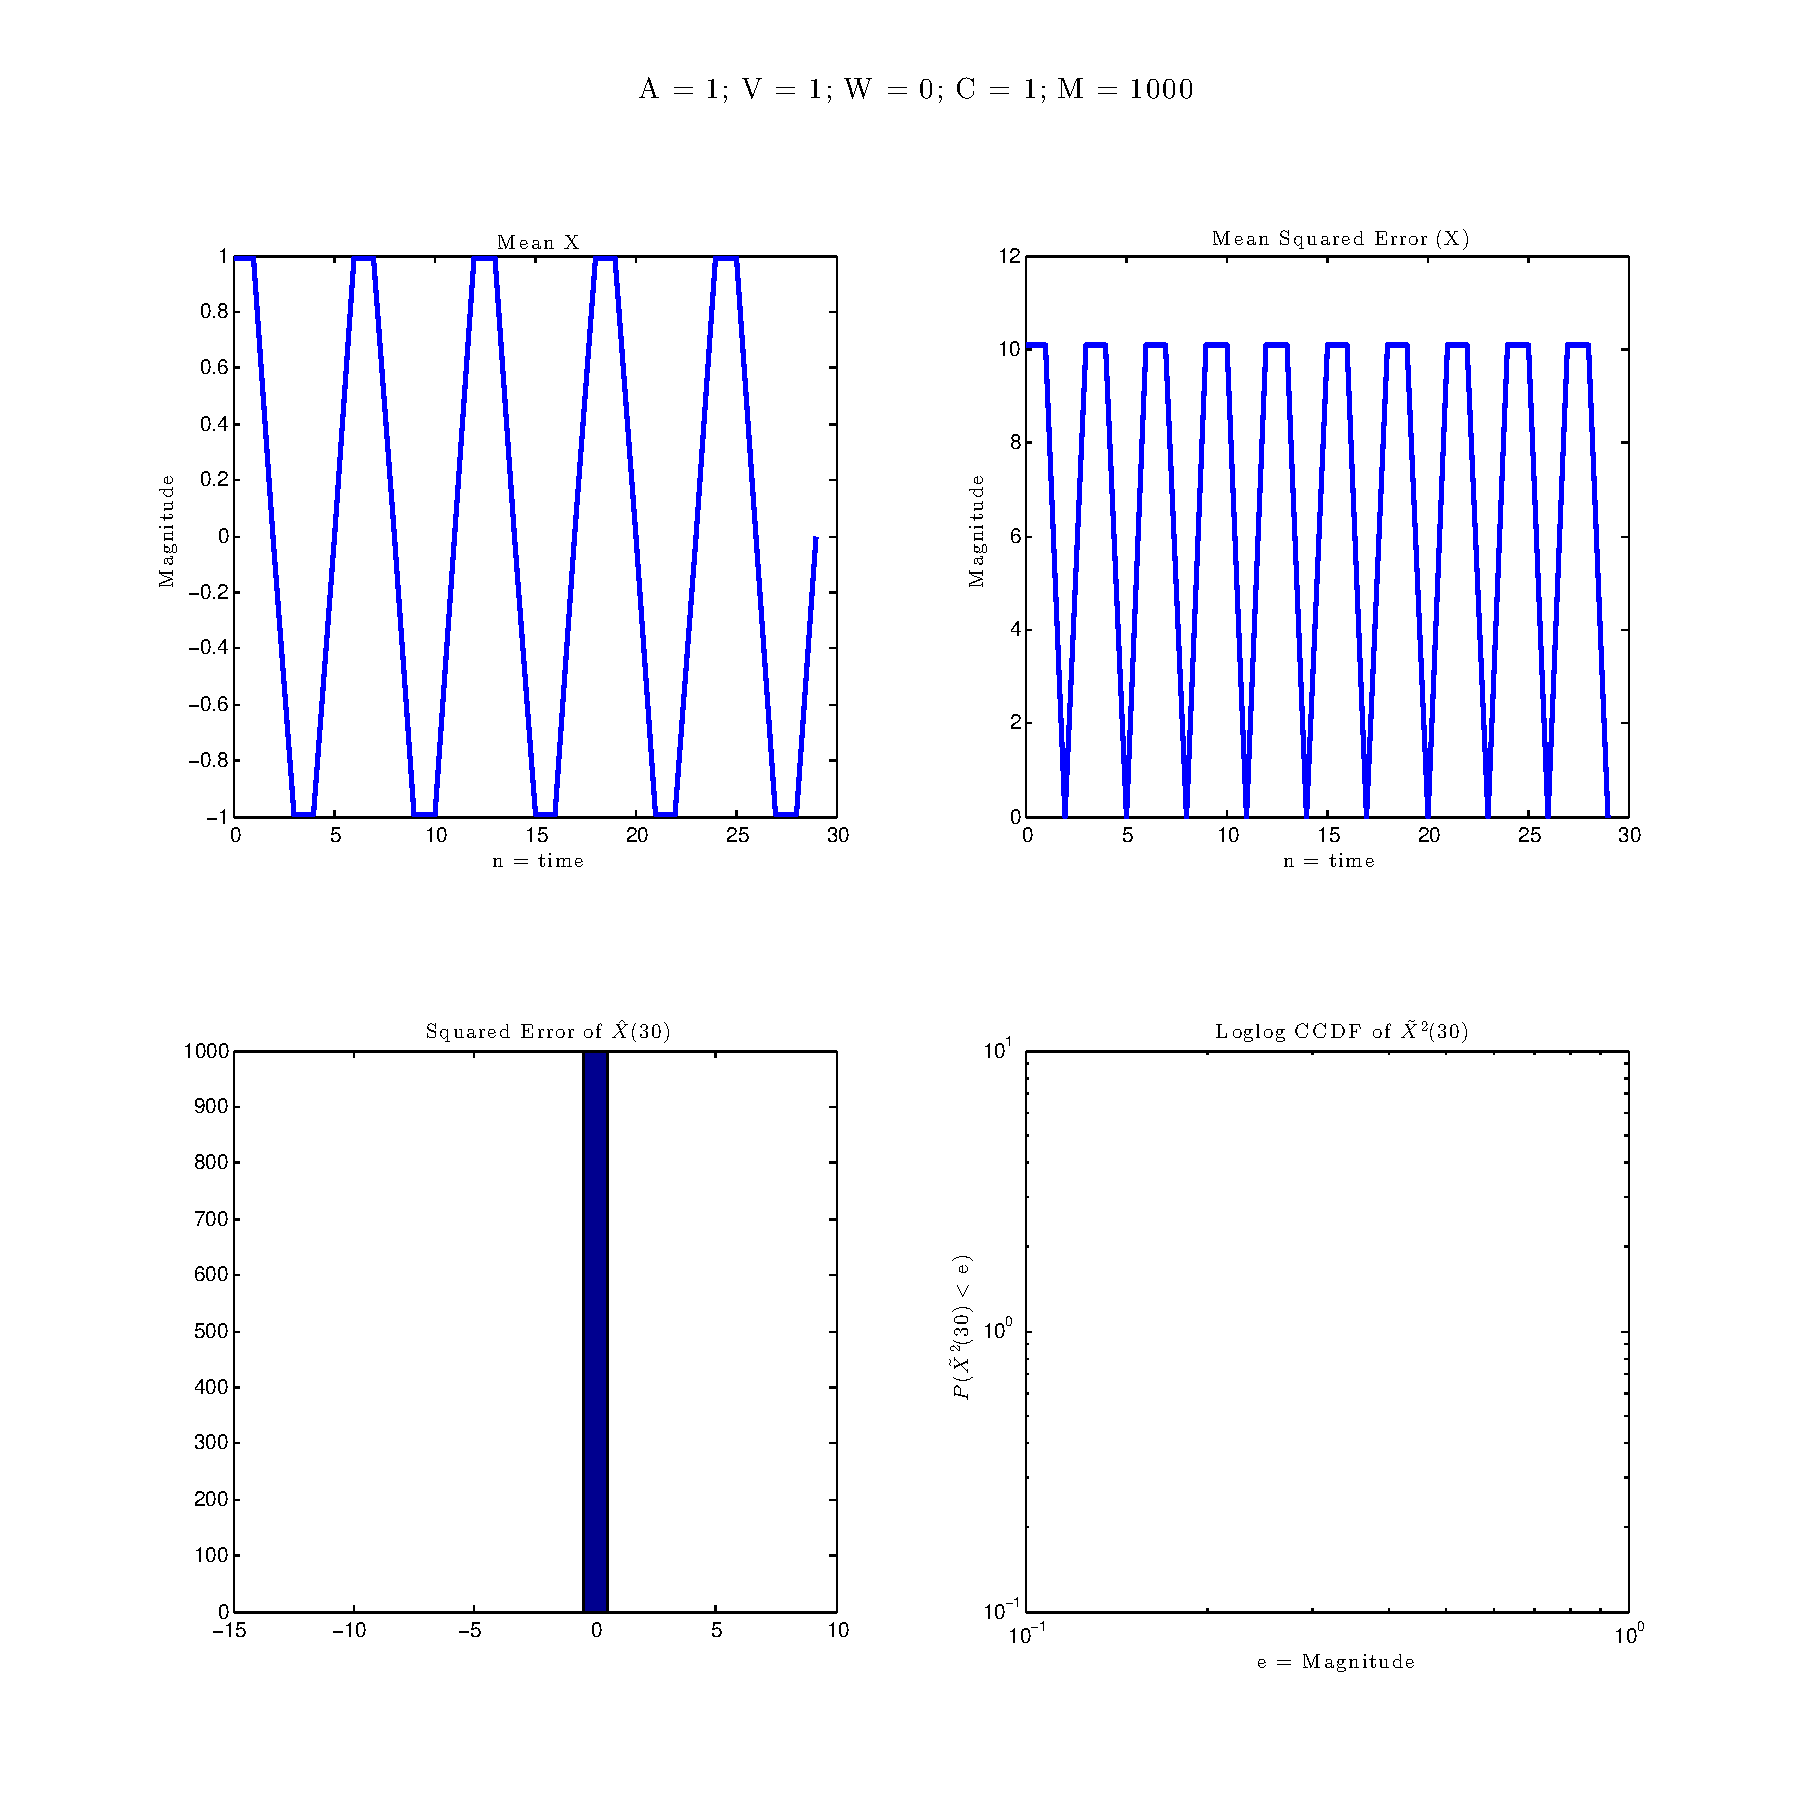
\includegraphics[width=0.5\textwidth]{udelay_6}\end{center}
We expect it to be sinusoidal because 1) In an AR model, when the first $\phi$ term is positive and the second $\phi$ term is negative, the system oscillates and 2) the control is effective, but because of delay in the next timestep the old control introduces new noise.

Even if $a < 1$, if state noise is introduced the noise terms will explode:
\begin{center}
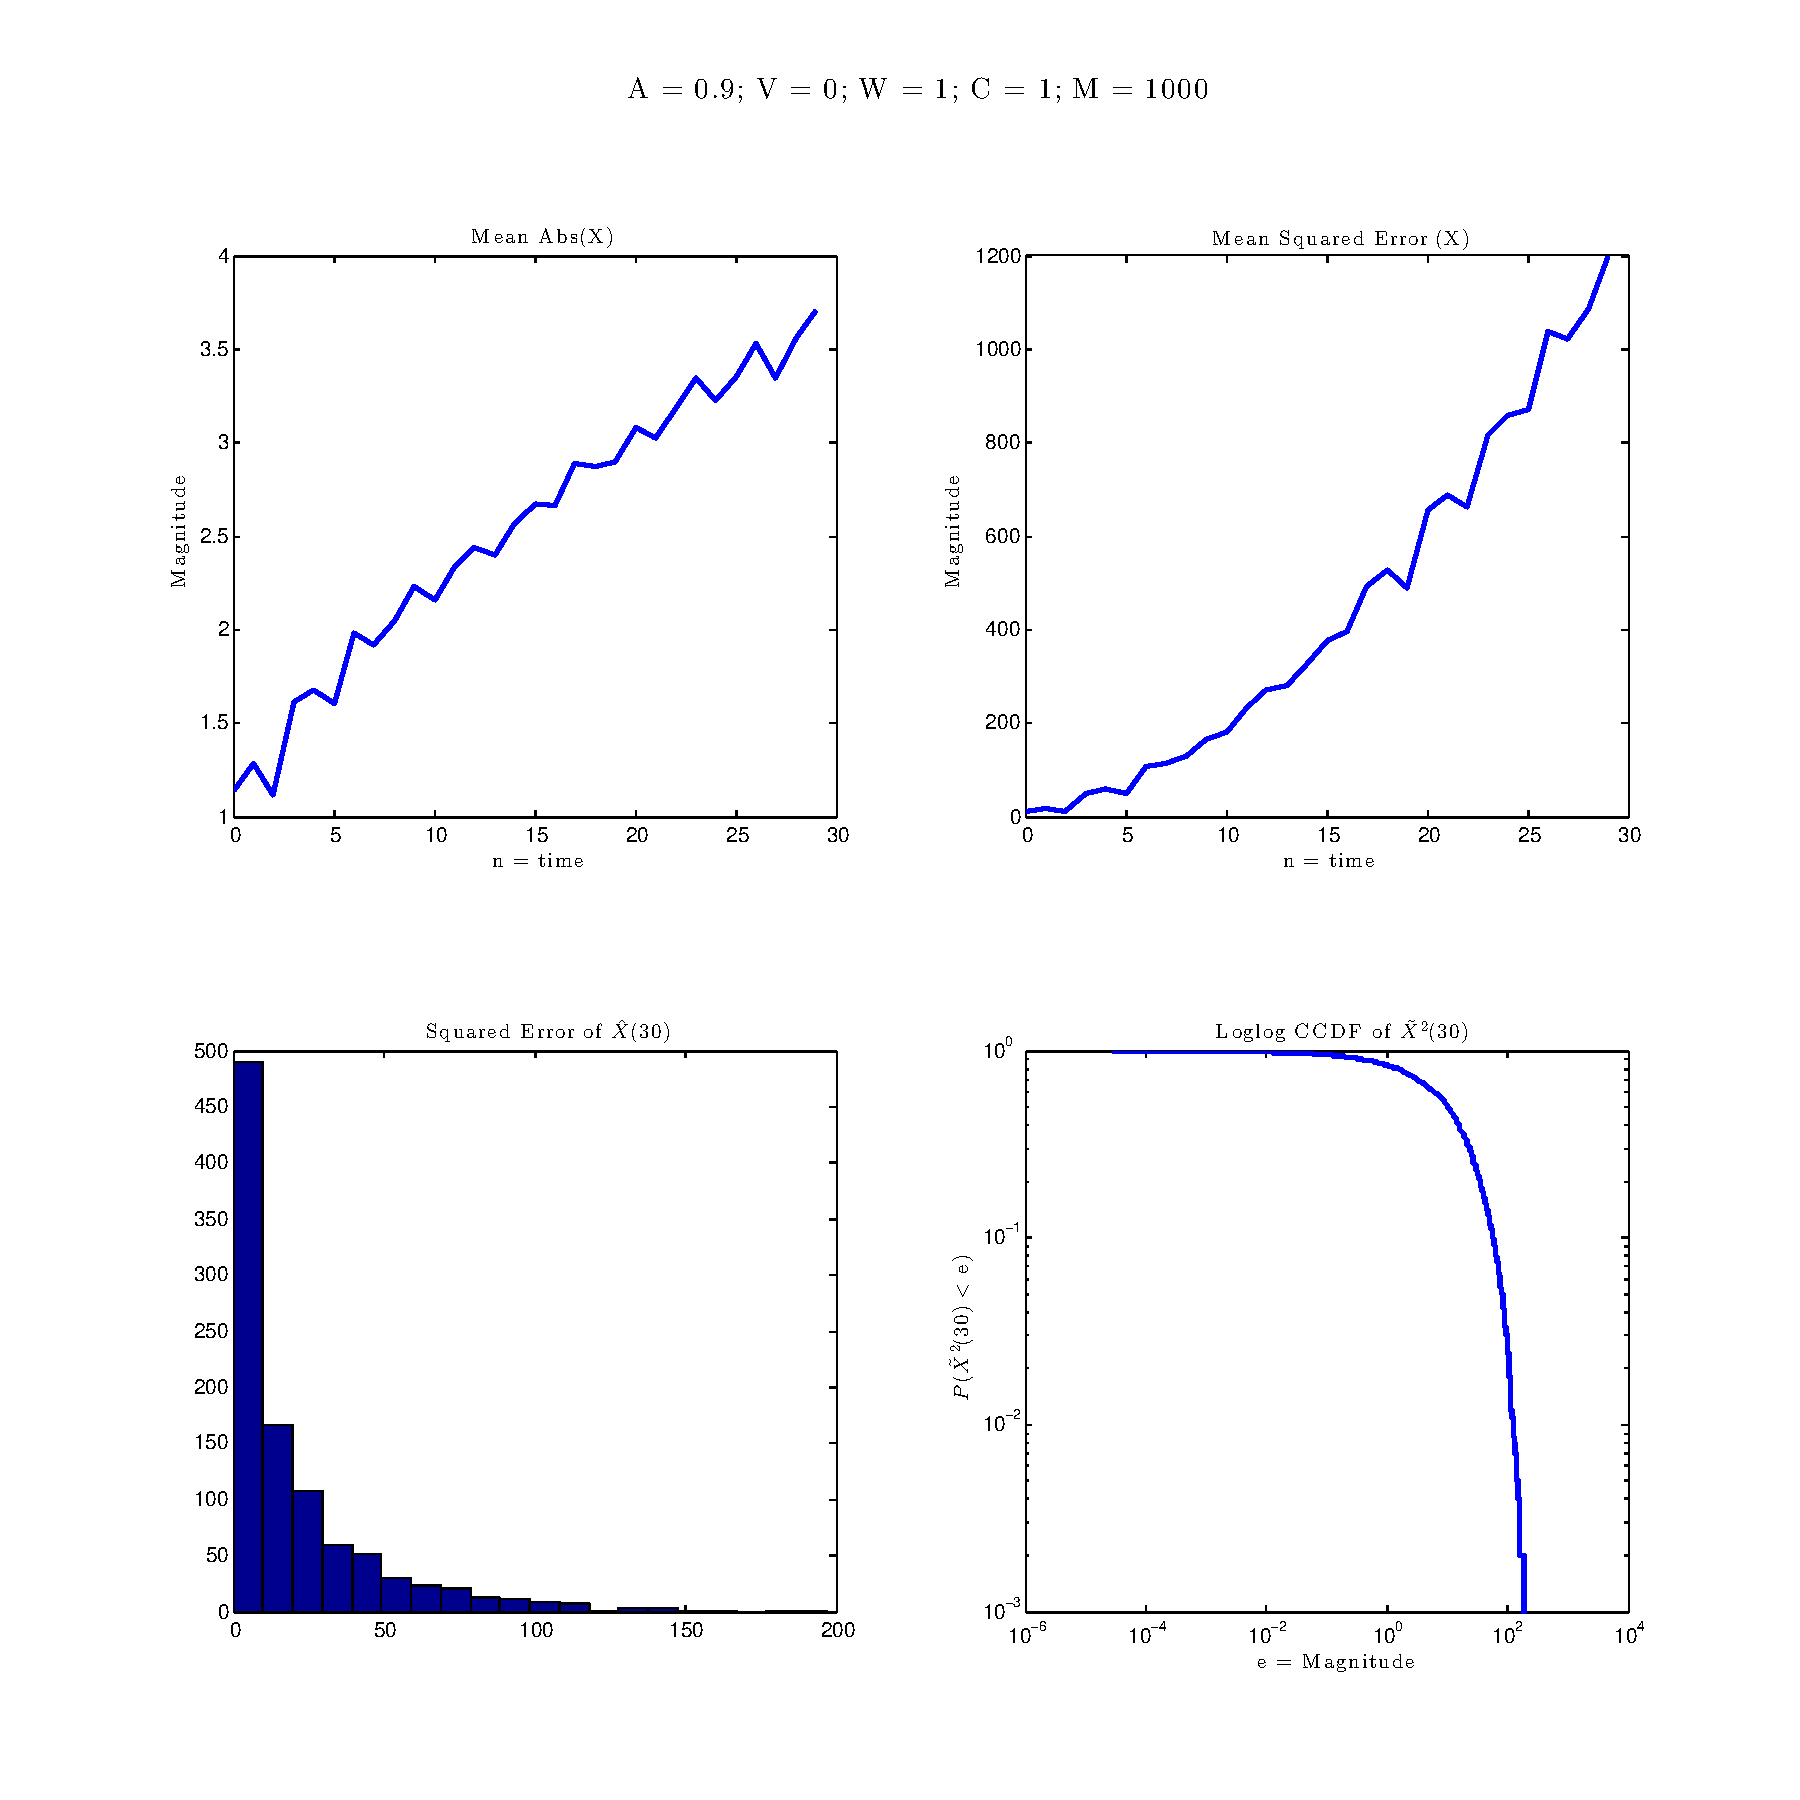
\includegraphics[width=0.5\textwidth]{udelay_4}
\end{center}

This is true no matter how small the state noise is:
\begin{center}
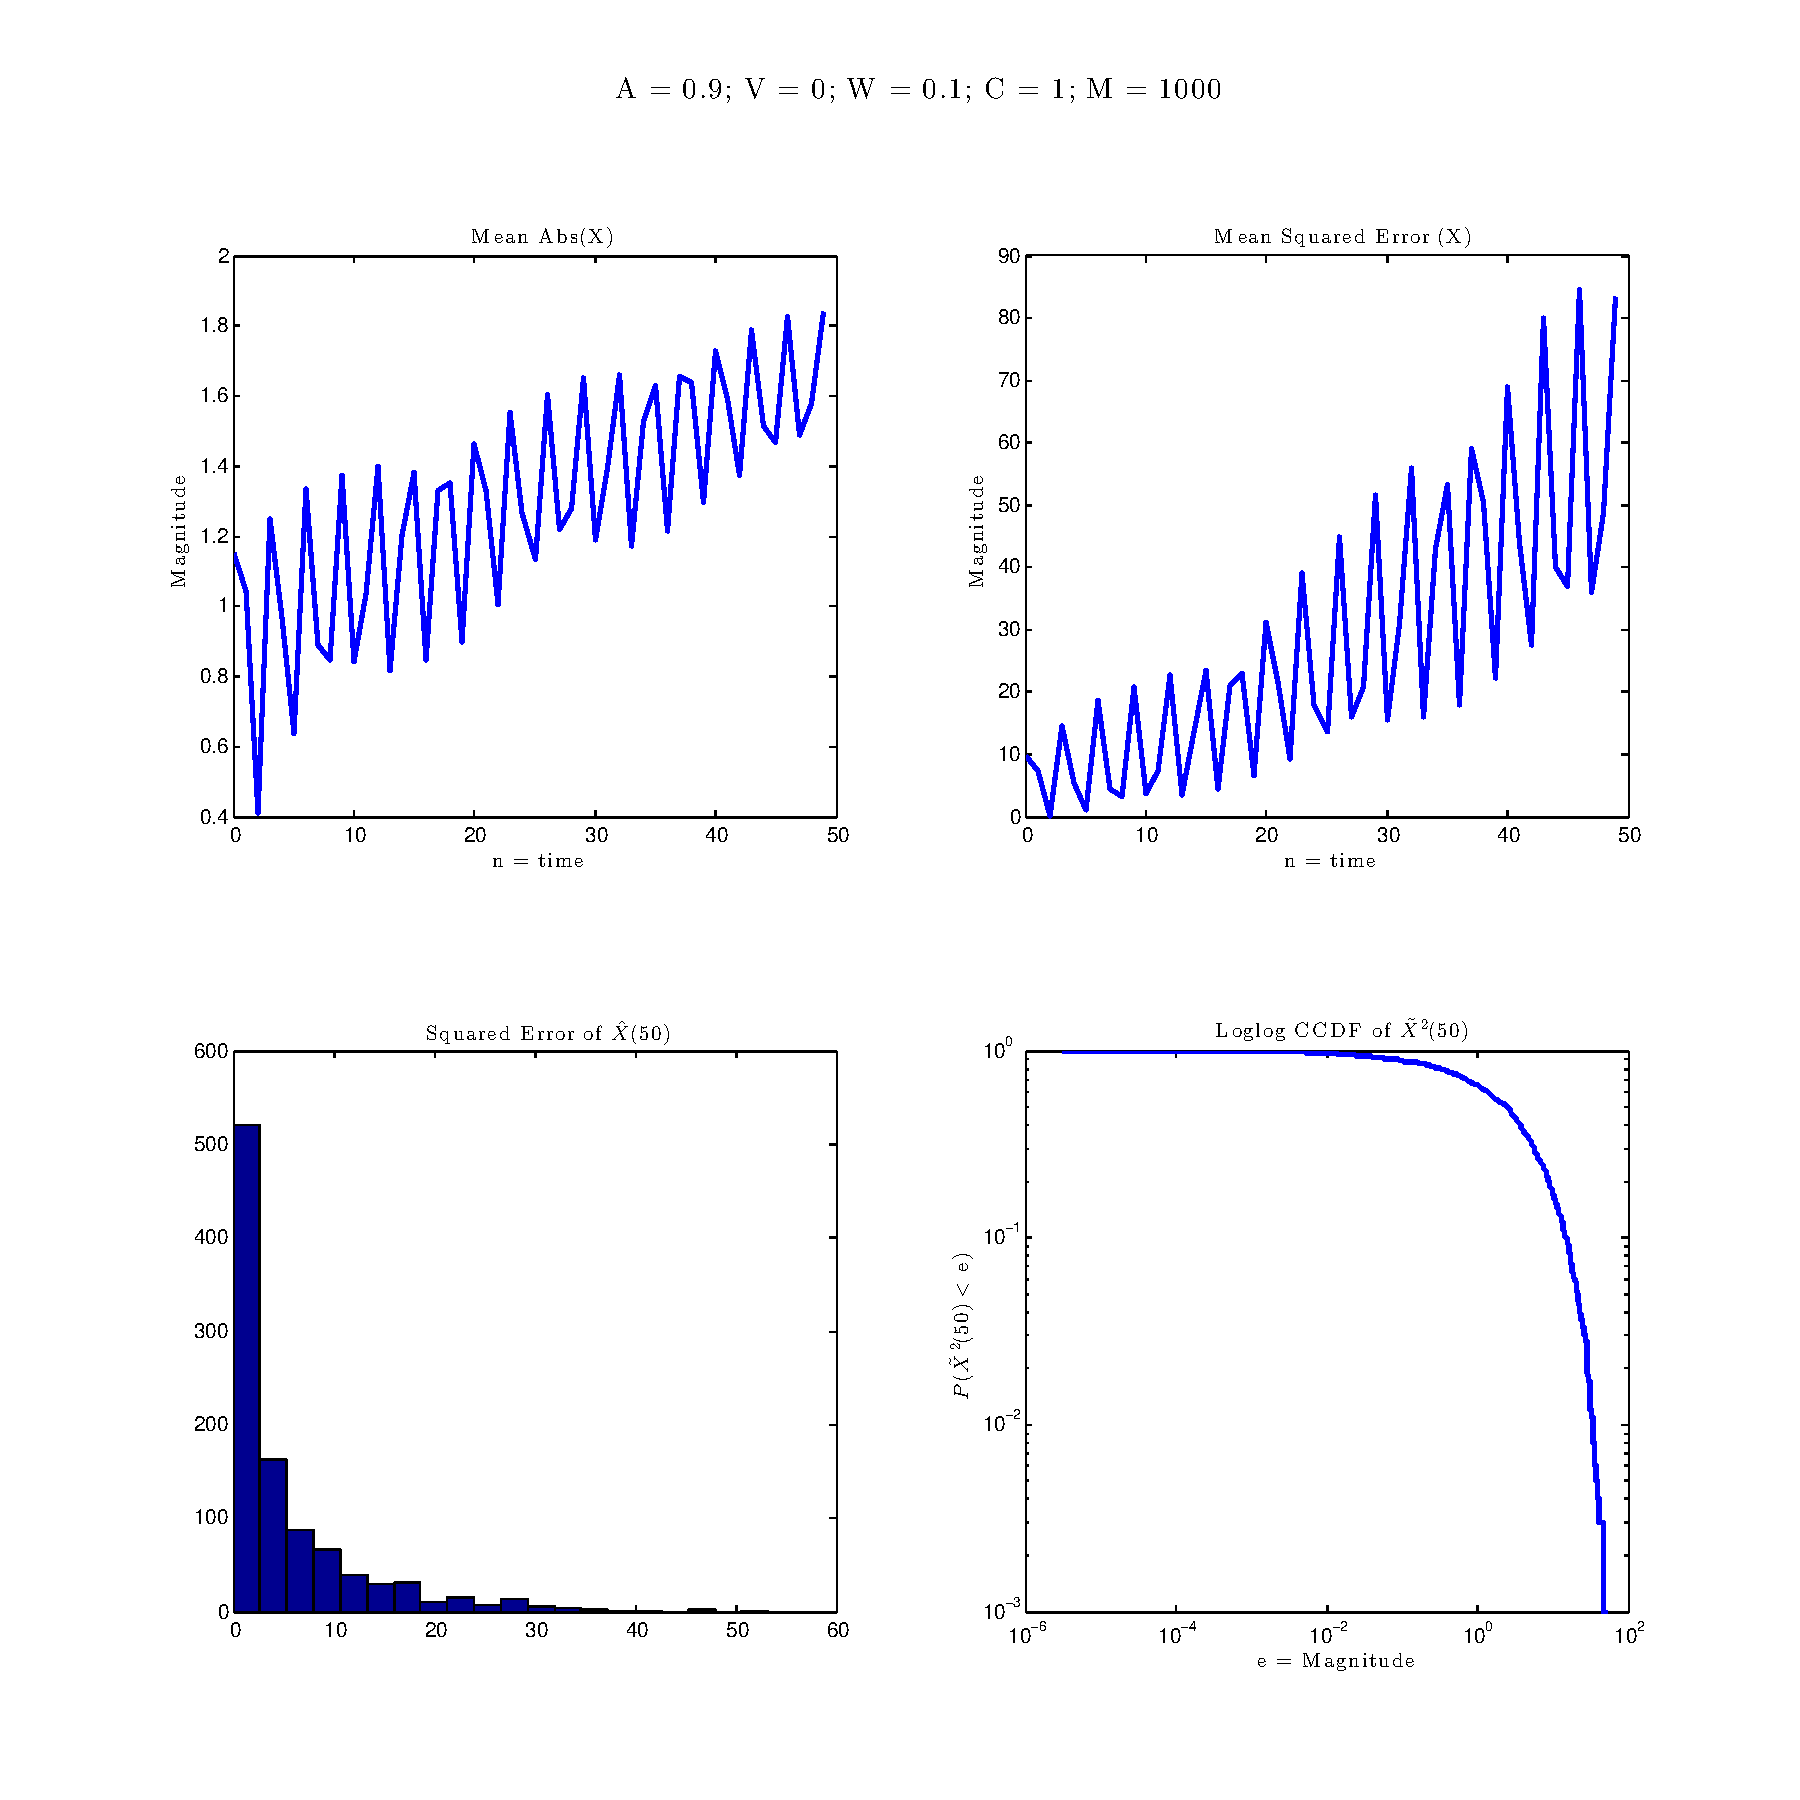
\includegraphics[width=0.5\textwidth]{udelay_5}
\end{center}

This is probably true because new noise is introduced at each timestep, and since the controller can't completely kill old noise there's no way to bound the amount of noise.

The calculations for observation noise would be involved because it appears difficult to find a recursive pattern for calculations of the control (similar to control with memory, observation noise would lead to an increasing number of terms to deal with.) 

\end{document}